\documentclass[12pt,a4paper]{report}
\usepackage[english]{babel}
\usepackage[utf8x]{inputenc}
\usepackage{newlfont}
\usepackage{color}
\usepackage{hyperref}
\usepackage{amsmath}
\usepackage{graphicx}
\usepackage{epigraph}
\usepackage[overload]{empheq}
\usepackage[inline, shortlabels]{enumitem}
\usepackage{bm}
\usepackage{color}
\usepackage{natbib}
\usepackage{float}
\usepackage{textcomp}

\usepackage{listings}

\definecolor{codegreen}{rgb}{0,0.6,0}
\definecolor{codegray}{rgb}{0.5,0.5,0.5}
\definecolor{codepurple}{rgb}{0.58,0,0.82}
\definecolor{backcolour}{rgb}{0.95,0.95,0.92}

\lstdefinestyle{snippet}{
    backgroundcolor=\color{backcolour},
    commentstyle=\color{codegreen},
    keywordstyle=\color{magenta},
    numberstyle=\tiny\color{codegray},
    stringstyle=\color{codepurple},
    basicstyle=\ttfamily\footnotesize,
    breakatwhitespace=false,
    breaklines=true,
    captionpos=t,
    keepspaces=true,
    numbers=left,
    numbersep=5pt,
    showspaces=false,
    showstringspaces=false,
    showtabs=false,
    tabsize=2
}

\usepackage{emptypage} % remove header in blanck pages

\usepackage[a4paper,top=4cm,bottom=4cm,left=3cm,right=3cm,marginparwidth=1.75cm]{geometry}

\hypersetup{
colorlinks,
citecolor=black,
filecolor=black,
linkcolor=black,
urlcolor=blue
}

\textwidth=450pt\oddsidemargin=0pt

\begin{document}
\begin{titlepage}
%
%
% ONCE YOU ARE FINISHED WITH YOUR CHANGES MODIFY "RED" WITH "BLACK" IN ALL \textcolor COMMENTS
%
%
\begin{center}
{{\Large{\textsc{Alma Mater Studiorum $\cdot$ University of  Bologna}}}} 
\rule[0.1cm]{15.8cm}{0.1mm}
\rule[0.5cm]{15.8cm}{0.6mm}
\\\vspace{3mm}
{\small{\bf School of Science \\
Department of Physics and Astronomy\\
Master Degree in Physics}}
\end{center}

\vspace{17mm}

\begin{center}
%
% INSERT THE TITLE OF YOUR THESIS
%
{\LARGE{\bf OPTIMIZATION AND APPLICATIONS\\
OF DEEP LEARNING ALGORITHMS\\
\vspace{3mm}
FOR SUPER-RESOLUTION IN MRI}}\\
\end{center}

\vspace{30mm} \par \noindent

\begin{minipage}[t]{0.47\textwidth}

{\large{\bf Supervisor: \vspace{2mm}\\
Prof. Gastone Castellani\\\\

\bf Co-supervisor:
\vspace{2mm}
\\
Dr. Nico Curti\\\\}}
\end{minipage}
%
\hfill
%
\begin{minipage}[t]{0.47\textwidth}\raggedleft \textcolor{black}{
{\large{\bf Submitted by:
\vspace{2mm}\\
Mattia Ceccarelli}}}
\end{minipage}

\vspace{40mm}

\begin{center}

Academic Year 2019/2020
\end{center}

\end{titlepage}

\newpage

\vspace*{125px}
\LARGE\textit{Abstract}
\normalsize
\vspace{2mm}

Abstract

\newpage
\normalsize 

\tableofcontents

\chapter{Introduction}

Brief introduction of the work

\section{Neural Network and Deep Learning}

A neural network is an interconnected structure of simple procedurals units, called nodes. Their functionality is inspired by the animals' brain and from the works on learning and neural plasticity of Donald Hebb \cite{hebb-learning}. From his book :

\begin{quote}
 \begin{center}
  \textit{Let us assume that the persistence or repetition of a reverberatory activity (or "trace") tends to induce lasting cellular changes that add to its stability.[…] When an axon of cell A is near enough to excite a cell B and repeatedly or persistently takes part in firing it, some growth process or metabolic change takes place in one or both cells such that A's efficiency, as one of the cells firing B, is increased}
 \end{center}
\end{quote}

which is an attempt to describe the change of strenght in neural relations as a consequence of stimulations.
From the so-called \textit{Hebbian Theory} rose the first computational models such as the \textit{Perceptron}, \textit{Neural Networks} and the modern \textit{Deep Learning}. 
The development of learning-based algorithms didn't catch up with the expected results until recently, mainly due to the exponential increase in available computational resources.

From a mathematical point of view, a neural network is a composition of non-linear multi-parametric functions. 
During the {\it training phase} the model tunes its parameters, starting from random ones, by minimizing the error function (called also loss or cost). 
Infact, machine learning problems are just optimization problems where the solution is not given in an analytical form, therefore trough iteratives techniques (generally some kind of gradient descent) we progressively approximate the correct result.

In general, there are 3 different kind of approach to learning:

\begin{itemize}
 \item {\bf supervised} It exists a labeled dataset in which the relationship between features (input) and expected output is known. 
 During training, the model is presented with many examples and it corrects its answers based on the correct response.  
 Some problems tied to supervised algorithms are classification, regression, object detection, segmentation and super-resolution.
 \item {\bf unsupervised} In this case, a labeled dataset does not exist, only the inputs data are available. 
 The training procedure must be tailored around the problem under study. Some examples of unsupervised algorithms are clustering, autoencoders, anomaly detection.
 \item {\bf reinforced} the model interacts with a dynamic environment and tries to reach a goal (e.g. winning in a competitive game). 
 For each iteration of the training process we assign a reward or a punishent, relatively to the progress in reaching the objective.
\end{itemize}

This work will focus on models trained using labeled samples, therefore in a supervised environment.

\subsection*{Perceptron}

The Perceptron (also called \textit{artificial neuron}) is the fundamental unit of every neural network and it is a simple model for a biological neuron, based on the works of Rosenblatt \cite{perceptron}. 
The \textit{perceptron} receives $N$ input values $x_1, x_2, ... x_N$ and the output is just a linear combination of the inputs plus a bias :

\begin{equation}
y = \sigma(\sum_{k=1}^N w_kx_k + w_0)
\end{equation}

where $\sigma$ is called \textit{activation function} and $w_0, w_1, ... w_N$ are the trainable weights.

Originally, the activation function was the \textit{Heaviside step function} whose value is zero for negative arguments and one for non-negative arguments: 

\begin{equation}
H(x) := 
\begin{cases}
  0 \text{ if } x < 0 \\ 
  1 \text{ if } x \geq 0 \\
\end{cases}
\end{equation}

In this case the perceptron is a \textit{linear discriminator} and as such, it is able to learn an hyperplane which linearly separates two set of data.
The weights are tuned during the training phase following the given update rule, usually :

\begin{equation}
 \bm{w}_{n+1} = \bm{w}_n + \eta (t - y)\bm{x}
 \label{eq:perceptron}
\end{equation}

where $\eta$ is the learning rate ($\eta \in [0,1]$) and $t$ is the true output. If the input instance is correctly classified,  the error $(t - y)$ would be zero and no weight is changed. 
Otherwise, the hyperplane is moved towards the misclassified example. 
Repeating this process will lead to a convergence only if the two classes are linearly separable.  

\subsection*{Fully Connected Structure}

The direct generalization of a simple perceptron is the \textit{Fully Connected Artificial Neural Network} (or {\it Multy Layer Perceptron}). 
It is composed by many Perceptron-like units called nodes, any one them performs the same computation as formula \ref{eq:perceptron} and \textit{feed} their output \textit{forward} to the next layer of nodes. 
A typical representation of this type of network is shown in figure \ref{fig:ann}:

\begin{figure}[h]
 \centering
 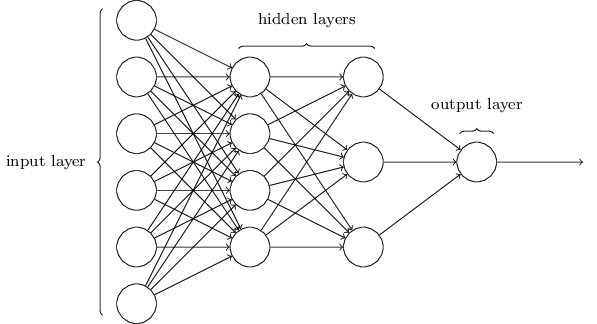
\includegraphics[scale=0.5]{./images/neural_net.png}
 \caption{{\it A common representation of a neural network: a single node works as the perceptron described above.}}
 \label{fig:ann}
\end{figure}

While the number of nodes in the input and output layers is fixed by the data under analysis, the best configuration of hidden layers is still an open problem.

The mathematical generalization from the perceptron is simple, indeed given the $i$-th layer its output vector $\bm{y}_i$ reads:  

\begin{equation}
 \bm{y}_i = \sigma(W_i \bm{y}_{i-1} + \bm{b}_i)
\end{equation}

where $W_i$ is the weights matrix of layer $i$ and $\bm{b}_i$ is the $i$-th bias vector, equivalent to $w_0$ in the perceptron case.
The output of the $i$-th layer becomes the input of the next one until the output layer yields the network's answer. 

As before, $\sigma$ is the activation function which can be different for every node, but it usually differs only from layer to layer. 
The choice of the best function for a given problem is still an open issue.

In a supervised environment, the model output is compared to the desired output ({\it truth}) by means of a cost function. 
An example of cost function is the sum of squared error : 

\begin{equation}
  C(W) = \frac{1}{N} \sum_{j=1}^{N} (y_j - t_j)^2
\end{equation}

where $N$ is the dimensionality of the output space. $C$ is considered as a function of the model's weights only since input data and true label $t$ are fixed.

{\bf overcome perceptron problems}

Those architectures are {\it universal approximators}, that means given an arbitrarly complex function, there is a fully connected neural network that can approximate it.

This type of network is called {\it feed forward} because the information flows linearly from the input to the output layer: however, it exists a class of models called {\it Recurrent} where this is not the case anymore and feedback loop are possible, but they are outside the scope of this work. 

\subsection*{Gradient Descent}

To minimize the loss function an update rule for the weights is needed. 
Given a cost funtion $C(w)$, the most simple one is the gradient descent:
\begin{equation}
 w \leftarrow w - \eta \nabla_w C
\end{equation}
The core idea is to modify the parameters by a small step in direction that minimize the error function. 
The lenght of the step is given by the {\it learning rate} $\eta$, which is a hyperparameter chosen by the user, while the direction of the step is given by $-\nabla_w C$, which point towards the steepest descent of the function landscape.

\begin{figure}[h]
 \centering
 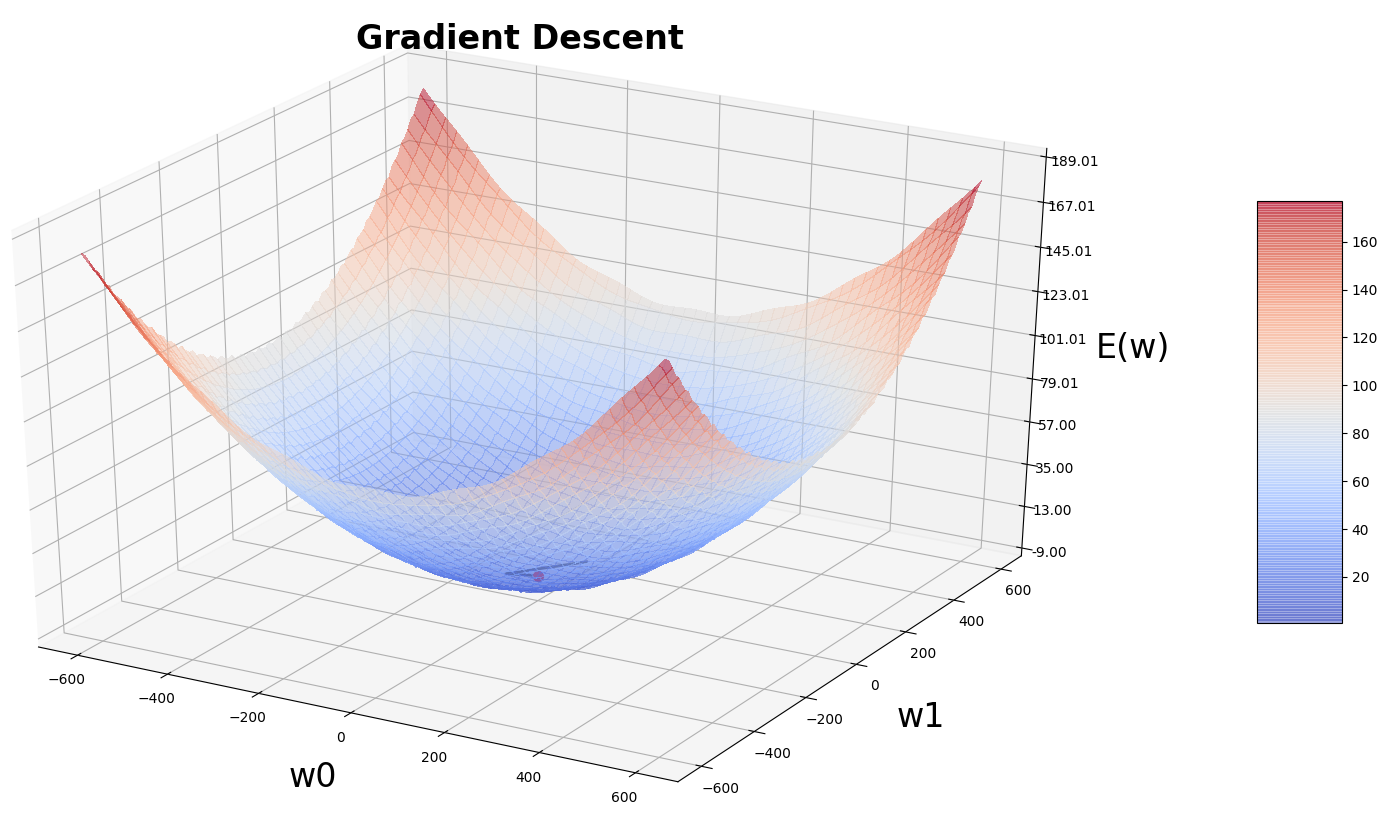
\includegraphics[scale=0.8]{./images/sgd.png}
 \label{fig:gd}
 \caption{\it Visual example of gradient descent for a model with 2 weights. The idea is to modify the weights to follow the direction of steepest descent for the landscape of the error function}
\end{figure}
The speed at which the algorithm converge to a solution and the precision of said solution are greatly influenced by the update rule. More complex and efficient update rules do exist, but they follow the same idea as the gradient descent.

\subsection*{Error Back Propagation}

The most common algorithm used to compute the updates to weights in the learning phase is the {\it Error Back Propagation}. 
Given a differentiable cost function $C(W)$, let's define :
\begin{align}
 \bm{z}_l &= W_l \bm{y}_{l-1} + \bm{b}_l  \\ 
 \bm{a}_l &= \sigma(\bm{z}_l)
\end{align}
respectively the de-activated and activated output vectors of layer $l$ for a model with $L$ total layer, and:
\begin{equation}
 \bm{\delta}_l = (\frac{\partial C}{\partial z_l^1}, \dots , \frac{\partial C}{\partial z_l^N}) 
\end{equation}
as the vector of errors of layer $l$. Then we can write the 4 equations of back propagation for the fully connected neural network \cite{neural-net-nielsen}:
\begin{align}
  &\bm{\delta}_L = \nabla_a C \odot \sigma'(\bm{z}_L) \\ 
  &\bm{\delta}_l = (W_{l+1}^T \bm{\delta}_{l+1}) \odot \sigma'(\bm{z}_l) \\
  &\frac{\partial C}{\partial b_l^j} = \delta_l^j \\
  &\frac{\partial C}{\partial w_l^{j k}} = a_{l-1}^k \delta_{l}^{j}
\end{align}
where  $\odot$ is the element-wise product.
Those equations can be generalized for others kind of layer, as I will show in the next chapters. 

The full training algorithm is : 

\begin{itemize}
 \setlength\itemsep{-0.3em}
 \item [-] define the model with random parameters
 \item [-] compute the output for one of the inputs
 \item [-] compute the loss function $C(W)$ and the gradients $\frac{\partial C}{\partial w_l^{j k}}$ and $\frac{\partial C}{\partial b_l^j}$ for each $l$.
 \item [-] updates the parameters following the update rule, 
 \item [-] iterate from step 2 until the loss is sufficiently small
\end{itemize}

\section{Super Resolution}

The term Super-Resolution (SR) referes to a class of techniques which aim is to enhance the spatial resolution of an image, thus converting a given low resolution (LR) image to a corresponding high resolution (HR) one, with better visual quality and refined details.
Image super-resolution is also called by other names like image scaling, interpolation, upsampling and zooming \cite{survey-sr}.
 {\bf FINISH}

\subsection*{Image Quality}

\cite{psnr_ssim}

\subsection*{PSNR}
\subsection*{SSIM}

\section{Magnetic Resonance}


\chapter{Algorithms}

Brief Intro to the works on algorithm (NumPyNet, Byron, Layers, )

\section{Byron}

Byron (Build YouR Own Neural network) is a novel Deep Learning framework written in C++. 

\section{NumPyNet}

\section{Convolutional Neural Network}

A Convolutional Neural Network (CNN) is a specialized kind of neural network for processing data that has known grid-like topology \cite{Goodfellow-et-al-2016}, like images, that can be considered as a grid of pixel.
The name indicates that at least one of the functions employed by the network is a convolution. In a continuos domain the convolution between two functions $f$ and $g$ is defined as: 
\begin{equation}
 (f * g)(t) = \int_{-\infty}^{+\infty} f(\tau)g(t-\tau)d\tau
\end{equation}
The first function $f$ is usually referred to as the input and the second function $g$ as kernel. 
For Image Processing applications we can define a 2-dimensional discrete version of the convolution in a finite domain using an image $I$ as input and a 2 dimensional kernel $k$:
\begin{equation}
 C[i, j] = \sum_{u=-N}^N \sum_{v=-M}^M k[u, v] \cdot I[i-u, j-v]
 \label{eq:conv}
\end{equation}
where $C[i, j]$ is the pixel value of the output image and $N$, $M$ are the kernel dimensions.
Practically speaking, a convolution is performed by sliding a kernel of dimension $N \times M$ over the image, each kernel position corresponds to a single output pixel, the value of which is calculated by multiplying together the kernel value and the underlaying pixel value for each cell of the kernel and summing all the results, as shown in figure \ref{fig:convolution}:

\begin{figure}[h]
 \centering
 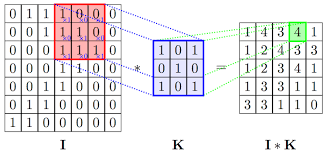
\includegraphics[scale=1.]{./images/conv.png}
 \label{fig:convolution}
 \caption{\it Visual example of convolution of an image I 7x7 with a 3x3 kernel K.}
\end{figure}

The convolution operation is also called $filtering$. By chosing the right kernel (filter) it is possible to highlight different features. For this reason the convolution operation is commonly used in image analysis: some of the most common applications are denoising, edge detection and edge enhancement. 

\section{Layers}

As described above, a neural network can be considered as a composition of function: for this reasons every Deep Learning framework (e.g. Keras/Tensorflow, Pytorch, Darknet) implement each function as an independent object called {\it Layer}. In Byron and NumPyNet, each layer contains at least 3 methods:
\begin{itemize}
 \setlength\itemsep{-0.3em}
 \item {\bf forward} the forward method compute the output of the layer, given as input the previous output. 
 \item {\bf backward} the backward method is essential for the training phase of the model: indeed, it computes all the updates for the layer weights and backpropagates the error to the previous layers in the chain.
 \item {\bf update} the update method applies the given update rules to the layer's weights.
\end{itemize}
By stacking different kinds of layer one after another, it is possible to build 
complex models with tens of millions of parameters. 
For the purposes of this work, I'm going to describe layers used in super resolution, however, Byron is developed also for different applications (object detection, classification, segmentation, style transfer, Recurrent NN etc...) and as such, many more layers are available.   

\subsection*{Convolutional Layer}

The convolutional layer (CL) object is the most used layer in DL image analysis, therefore its implementation must be as efficient as possible.
Its purpose is to perform multiple (sometimes thousands) convolution over the input to extract different high-level features, which are compositions of many low-level attributes of the image (e.g edges, simple shapes).
In the brain/neuron analogy, every entry in the output volume can also be interpreted as an output of a neuron that looks at only a small region, the neuron's {\it receptive field} in the input and shares parameters with all the neuron spatially close.
As more CLs are stacked, the receptive field of a single neuron grows and with that, the complexity of the features it is able to extract.
The local nature of the receptive field allows the models to recognize features regardless of the position in the images. In other words, it is independent from translations \cite{Goodfellow-et-al-2016}. 

The difference from a traditional convolutional approach is that instead of using pre-determined filters, the network is supposed to learn its own.
A CL si defined by the following parameters: 

\begin{itemize}
 \setlength\itemsep{-0.2em}
 \item [-] {\bf kernel size} : it is the size of the sliding filters. The depth of the filters is decided by the depth of the input images (which is the number of channels.). The remanining 2 dimensions (widht and height) can be indipendent from one another, but most implementation require square kernels.
 \item [-] {\bf strides} : defines the movement of the filters. With a low stride (e.g. unitary) the windows tends to overlap. With highr stride values we have less overlap (or none) and the dimension of the output decrease.
 \item [-] {\bf number of filters} : is the number of different filters to apply to the input. It also indicates the depth of the output.
 \item [-] {\bf padding} : is the dimensions of an artificial enlargement of the input to allow the application of filters on borders. Usually, it can be interpreted as the number of rows/columns of pixel to add to the input, however some libraries (e.g Keras) consider it only as binary: in case is true, only the minimum number of rows/columns are appended to keep the same spatial dimension.
\end{itemize}
Given the parameters, it is straightforward to compute the number of weights and bias needed for the initialization of the CL: indeed, suppose an image of dimensions $(H, W, C)$ slided by $n$ different 3-D filters of size $(k_x, k_y)$ with strides $(s_x, s_y)$ and padding $p$, then:
\begin{align}
 \# weights &= n \times k_x \times k_y \times C \\
 \# bias &= n
\end{align}
Note that the number of weights does not depend on the input spatial size but only on its depth. It is important because a fully convolutional network can receives images of any size as long as they have the correct depth. Moreover, using larger inputs do not requires more weights, as is the case for fully connected structure. 

The output dimensions are $(out\_H, out\_W, n)$ where :
\begin{align}
 out\_H &= \lfloor\frac{H - k_x + p}{s_x}\rfloor + 1 \\
 out\_W &= \lfloor\frac{W - k_y + p}{s_y}\rfloor + 1
\end{align}

Even if the operation can be implemented as described above in equation \ref{eq:conv}, this is never the case: it is certainly easier but also order of magnitude slower than more common algorithms.
A huge speed up in performances is given by realising that a discrete convolution can be viewed as a single matrix multiplication. By performing a clever transformation of the input into a flat matrix, in which every columns yields the values that have to be multiplied by the filters for each output, as shown in figure \ref{fig:im2col}

\begin{figure}[h]
 \centering
 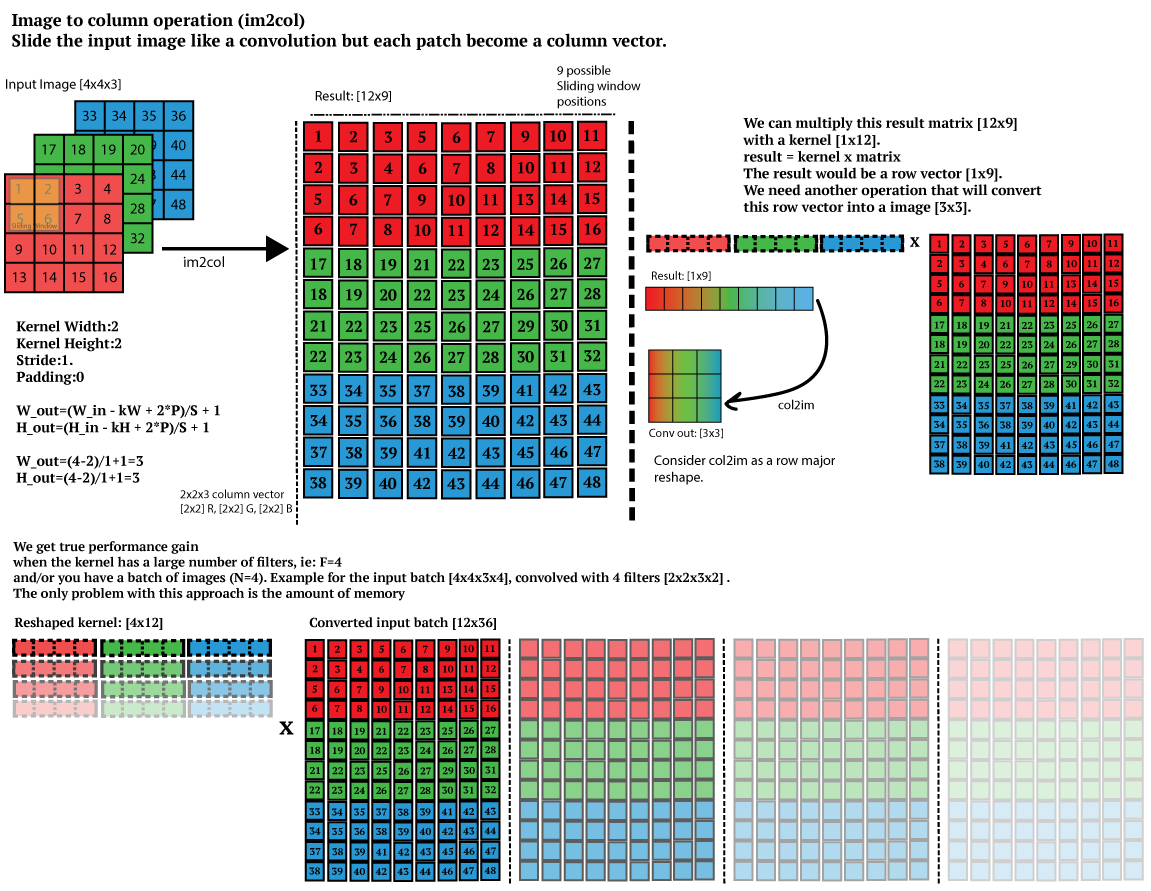
\includegraphics[scale=0.35]{./images/im2col.png}
 \label{fig:im2col}
 \caption{\it Scheme of the im2col algorithm using a $2 \times 2 \times 3$ filter with stride 1 on a $4 \times 4 \times 3$ image. The matrix multiplication is between a $n \times 12$ and a $12 \times 9$ matrixes.}
\end{figure}

This re-arrengement is commonly called im2col. The main downside is that a lot more memory is needed to store the newly arranged matrix.
The larger the number of kernels, the higher is the time gain of this implementation over a naive one.  

Another important optimization comes from linear algebra considerations and is called {\it Coppersmith-Winograd algorithm}, which was designed to optimize the matrix product.
Suppose we have an input image of just 4 elements and a 1-D filter mask with size 3:

\begin{equation}
\mbox{img} = \left[\begin{array}{cccc} d0 & d1 & d2 & d3 \end{array}\right] \quad\quad \mbox{weights} = \left[\begin{array}{ccc} g0 & g1 & g2 \end{array}\right]
\end{equation}
\\
we can now use the \textsf{im2col} algorithm previously described and reshape our input image and weights into

\begin{equation}
\mbox{img} = \left[
\begin{array}{ccc}
d0 & d1 & d2 \\
d1 & d2 & d3
\end{array}
\right],
\quad\quad
\mbox{weights} = \left[
\begin{array}{c}
g0 \\
g1 \\
g2
\end{array}
\right]
\end{equation}
\\
given this data, we can simply compute the output as the matrix product of this two matrices:

\begin{equation}
\mbox{output} = \left[
\begin{array}{ccc}
d0 & d1 & d2 \\
d1 & d2 & d3
\end{array}
\right]
\left[
\begin{array}{c}
g0 \\
g1 \\
g2
\end{array}
\right] = \left[
\begin{array}{c}
d0 \cdot g0 + d1 \cdot g1 + d2 \cdot g2 \\
d1 \cdot g0 + d2 \cdot g1 + d3 \cdot g2 
\end{array}
\right]
\end{equation}
\\
The Winograd algorithm rewrites this computation as follow:

\begin{equation}
\mbox{output} = \left[
\begin{array}{ccc}
d0 & d1 & d2 \\
d1 & d2 & d3
\end{array}
\right]
\left[
\begin{array}{c}
g0 \\
g1 \\
g2
\end{array}
\right] = \left[
\begin{array}{c}
m1 + m2 + m3 \\
m2 - m3 - m4
\end{array}
\right]
\end{equation}
\\
where

\begin{equation}
\begin{aligned}
m1 = (d0 - d2)g0\quad\quad m2 = (d1 + d2)\frac{g0 + g1 + g2}{2}
\\
m4 = (d1 - d3)g2\quad\quad m3 = (d2 - d1)\frac{g0 - g1 + g2}{2}
\end{aligned}
\end{equation}

The two fractions in $m2$ and $m3$ involve only weight's values, so they can be computed once per filter. Moreover, the normal matrix multiplication is composed of 6 multiplications and 4 addition, while the winograd algorithm reduce the number of multiplication to 4, that is very significant, considering that a  single multiplication takes 7 clock-cycles and an addition only 3. 
In Byron we provide the winograd algorithm for square kernels of size 3 and stride 1, since it is one of the most common combinations in Deep Learning and the generalization is not straightforward.

\begin{itemize}
 \item col2im backward
\end{itemize}
 
\subsection*{Pooling}

Pooling operations are down-sampling operations, so that the spatial dimensions of the input are reduced. Similarly to what happens in a CL, in pooling layers a 3-D kernel of size $k_x \times k_y \times C$ slides across an image of size $H \times W \times C$, however the operation performed by this kind of layers is fixed and does not change during the course of training.
The two main pooling functions are max-pooling and average-pooling: as suggested by the names, the former  
returns the maximum value of every window of the images super-posed by the kernel, as shown in figure \ref{fig:maxpool}:

\begin{figure}[h]
 \centering
 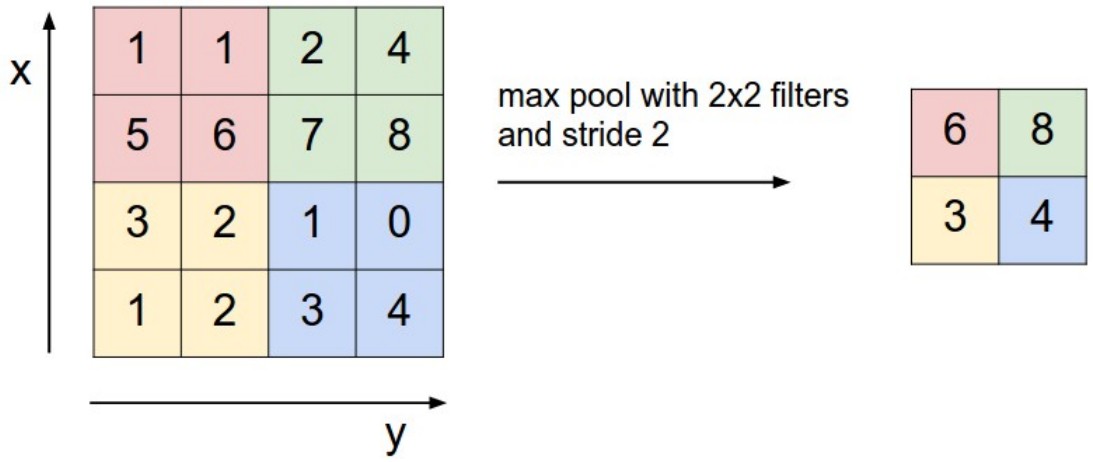
\includegraphics[scale=0.35]{./images/maxpool.png}
 \label{fig:maxpool}
 \caption{\it Scheme of maxpool operations with a kernel of size $2 \times 2$ and stride $2$ over an image of size $4 \times 4$. Picture from CS231n}
\end{figure}

The latter instead, returns the average value of the window and can be seen as a convolution where every weight in the kernel is $\frac{1}{k_x \cdot k_y}$.
The results expected from an Average pooling operations are shown in figure \ref{fig:avgpool:ex}:

\begin{figure}[h]
 \centering
 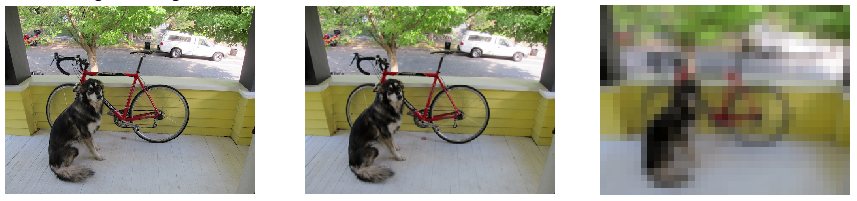
\includegraphics[scale=0.7]{./images/avgpool_layer.png}
 \label{fig:avgpool:ex}
 \caption{\it Average pooling applied to a test image: (left) the original image, (center) average pooling with a $3 \times 3$ kernel, (right) average pooling with a $30 \times 30$ kernel. The images have been obtained using NumPyNet}
\end{figure}

Other popular pooling functions include the $L^2$ norm of a rectangular neighborhood or a weighted average based on the distance from the central pixel.

A typical block of a convolutional network consists of three stages: In the first stage a CL performs several convolutions in parallel, in the second stage each convolution result is run through a non-linear activation function (sometimes called {\it detector}) and in the third stage a pooling function is used to further modify the output. 
The modification brought by pooling is helpful in different ways: first of all, it is a straightforward computational performance improvement, since less features also means less operations. 
Moreover, in all cases, pooling helps to make representation approximately invariant to small translation of the input and invariance to local translation can be a useful property if the objective is to decide wether a feature is present rather than where it is located \cite{Goodfellow-et-al-2016}.
The reductions of features can also prevent over-fitting problems during training, improving the general performances of the model. 

A pooling layer is defined by the same parameters as a CL, minus the number of filters:

\begin{itemize}
 \setlength\itemsep{-0.2em}
 \item [-] {\bf kernel size} : it is the size of the sliding filters. The depth of the filters is decided by the depth of the input images (which is the number of channels.). The remanining 2 dimensions (widht and height) can be indipendent from one another, but most implementations require square kernels.
 \item [-] {\bf strides} : defines the movement of the filters. With a low stride (e.g. unitary) the windows tends to overlap. With higher stride values we have less overlap (or none) and the dimension of the output decrease. Usually pooling operations have a stride of 2.
 \item [-] {\bf padding} : is the dimensions of an artificial enlargement of the input to allow the application of filters on borders. Usually, it can be interpreted as the number of rows/columns of pixel to add to the input, however some libraries (e.g Keras) consider it only as binary: in case is true, only the minimum number of rows/columns are appended to keep the same spatial dimension. Most often than not, no padding is applied during pooling operations.
\end{itemize}

The output dimensions for Pooling layers are the same as for CLs, however, since the operations does not change during the training phase, they have no weights.

Due to the similarities with the CL it is possible to implement a pooling layers through the im2col algorithm, as an example, the NumPyNet implementation shown in the snippet below make use of the function \texttt{asStride} to create a \texttt{view} of the input array: 

\lstset{style=snippet}
\begin{lstlisting}[language=Python, caption=NumPyNet version of AvgPool function, label=code:py_avgpool]
import numpy as np

class Avgpool_layer(object):

  def __init__(self, size=(3, 3), stride=(2, 2)):

    self.size = size
    self.stride = stride
    self.batch, self.w, self.h, self.c = (0, 0, 0, 0)
    self.output, self.delta = (None, None)

  def _asStride(self, input, size, stride):

    batch_stride, s0, s1 = input.strides[:3]
    batch,        w,  h  = input.shape[:3]
    kx, ky     = size
    st1, st2   = stride

    # Shape of the final view
    view_shape = (batch, 1 + (w - kx)//st1, 1 + (h - ky)//st2) + input.shape[3:] + (kx, ky)

    # strides of the final view
    strides = (batch_stride, st1 * s0, st2 * s1) + input.strides[3:] + (s0, s1)

    subs = np.lib.stride_tricks.as_strided(input, view_shape, strides=strides)
    # returns a view with shape = (batch, out_w, out_h, out_c, kx, ky)
    return subs

  def forward(self, input):

    self.batch, self.w, self.h, self.c = input.shape
    kx, ky = self.size
    sx, sy = self.stride

    input = input[:, : (self.w - kx) // sx*sx + kx, : (self.h - ky) // sy*sy + ky, ...]
    # 'view' is the strided input image, shape = (batch, out_w, out_h, out_c, kx, ky)
    view = self._asStride(input, self.size, self.stride)

    # Mean of every sub matrix, computed without considering the pad(np.nan)
    self.output = np.nanmean(view, axis=(4, 5))

\end{lstlisting}

A \texttt{view} is a special \texttt{numpy} object which retains the same information of the original array arranged in a different way, but without occupying more memory. In this case, the re-arrengement is very similar to an im2col, with the only differece that we are not bound to any number of dimensions. The resulting tensor has indeed 6 dimensions.
Since no copy is produces in this operation we can obtain a faster execution.

In pooling layer the backward function is similar to what we saw for convolutional layers, this time we don't have to compute the weights updates though, only the error to backprogate along the network.
For maxpool layers, only the maximum input pixel for every window is involved in the backward pass. Indeed, if we consider the simple case in which the forward function is : 

\begin{equation}
 m = max(a, b)
\end{equation}

and, as described in the dedicated chapter, we know that $\frac{\partial C}{\partial m}$ is the error passed back from the next layer: the objective is to compute $\frac{\partial C}{\partial a}$ and $\frac{\partial C}{\partial b}$. 
If $a > b$ we have : 

\begin{equation}
 m = a \quad \Rightarrow \quad \frac{\partial C}{\partial m} = \frac{\partial C}{\partial a}
\end{equation}
$m$ does not depends on $b$ so $\frac{\partial C}{\partial b} = 0$.

{\bf FINISH}

% According to \cite{nopool}, it is possible to build models exclusively out of convolutional layers without the need for pooling and reach state-of-the art performances 

\subsection*{Shortcut Connections}

An important advancement in network architecture has been brought by the introduction of Shortcut (or Residual) Connections \cite{residual}. Famously, ciao

instead of learning a function $F(x)$ we try to learn $F(x) + x$

\subsection*{Pixel Shuffle}
\subsection*{Batch Normalization}
\subsection*{Activations}
\subsection*{Loss Function}
\section{Timing}
\section{}

\chapter{Dataset and Methodology}

\section{Dataset}

\section{Models}

\chapter{Results}


\newpage
\nocite{*}
\bibliographystyle{abbrv}
\bibliography{biblio}

\end{document}
